\documentclass[11pt,a4paper]{article}

\usepackage{amsmath,amssymb,amsthm}
\usepackage{mathtools}
\usepackage{geometry}
\usepackage{hyperref}
\usepackage{xcolor}
\usepackage{tikz}
\usetikzlibrary{arrows.meta,positioning,decorations.markings,calc}
\usepackage{tcolorbox}
\tcbuselibrary{skins,breakable}
\usepackage{enumitem}
\usepackage{microtype}
\usepackage{booktabs}

\geometry{margin=2.3cm}

\hypersetup{colorlinks=true,linkcolor=blue!60!black,urlcolor=blue!60!black}

\definecolor{gunnaryellow}{RGB}{255,236,179}
\definecolor{gunnarpink}{RGB}{255,182,205}
\definecolor{gunnarblue}{RGB}{170,210,240}
\definecolor{commentboxbg}{RGB}{240,245,250}

\newtcolorbox{commentbox}[1][]{
  colback=commentboxbg, colframe=blue!50!black,
  fonttitle=\bfseries, title=Commentary, breakable, #1
}

\newcommand{\hl}[1]{\colorbox{gunnaryellow}{$#1$}}
\newcommand{\hpink}[1]{\colorbox{gunnarpink}{$#1$}}
\newcommand{\hblue}[1]{\colorbox{gunnarblue}{$#1$}}

% --- DP diagram macros (1-loop): bubble (self-energy) + triangle (vertex) ---
\newcommand{\dpbubble}{%
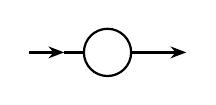
\begin{tikzpicture}[baseline=-0.5ex]
  \draw[thick,-{Stealth[length=2mm]}] (-1.0,0)--(-0.55,0);
  \draw[thick] (-0.55,0)--(-0.3,0);
  \draw[thick] (0,0) circle (0.3);
  \draw[thick] (0.3,0)--(0.55,0);
  \draw[thick,-{Stealth[length=2mm]}] (0.55,0)--(1.0,0);
\end{tikzpicture}}

\newcommand{\dptriangle}{%
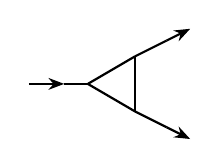
\begin{tikzpicture}[baseline=-0.5ex]
  % three-point vertex correction: triangle with one external in, two out
  \draw[thick,-{Stealth[length=2mm]}] (-1.05,0)--(-0.6,0);
  \draw[thick] (-0.6,0)--(-0.3,0);
  \draw[thick] (-0.3,0)--(0.3,0.35);
  \draw[thick] (-0.3,0)--(0.3,-0.35);
  \draw[thick] (0.3,0.35)--(0.3,-0.35);
  \draw[thick] (0.3,0.35)--(0.7,0.55);
  \draw[thick,-{Stealth[length=2mm]}] (0.7,0.55)--(1.0,0.7);
  \draw[thick] (0.3,-0.35)--(0.7,-0.55);
  \draw[thick,-{Stealth[length=2mm]}] (0.7,-0.55)--(1.0,-0.7);
\end{tikzpicture}}

\title{\large Note from Gunnar (1 May 2026): RG of DP --- exponents without explicit loops\\
\normalsize transcribed; reply lives in \texttt{reply.tex}}
\author{}
\date{}

\begin{document}
\maketitle
\vspace{-2.5em}

\section*{Preamble (Gunnar, in his own words)}

\begin{quote}
\itshape
I want to understand the claim of ``exponents without loop integrals'' a bit better.

In the case of Doi--Peliti I can see how this may work. But Claude seemed to suggest that
in the Gribov process (which is directed percolation) exponents are a matter of pure
combinatorics, which I don't see.

So now I will derive the exponents of directed percolation and it will become clear that
you get them without calculating integrals explicitly, although you need to know some of
their behaviour. So yes: \textbf{exponents without explicit loops, but no, nothing to do
with combinatorics}.

As an aside, I wonder whether analytic combinatorics can help characterising the wild
forest of diagrams you get when you attempt to write down $\varphi^4$-theory in
Doi--Peliti using a Hermite basis.
\end{quote}

\section*{DP --- to one loop}

To one loop there are two diagrams to be considered:

\begin{center}
\dpbubble \qquad\text{and}\qquad \dptriangle
\end{center}

\paragraph{Bubble (self-energy).} With symmetry factor $\tfrac{1}{2}\!\cdot\!2 = 1$,
\begin{align*}
\text{(bubble)}
&\;=\; 2 g^{2}\!\int\! \frac{d\omega'}{2\pi}\frac{d^{d}k'}{(2\pi)^{d}}\;
\frac{1}{-\mathrm i(\omega+\omega') + D(k+k')^{2} + r}\;\cdot\;
\frac{1}{\mathrm i\omega' + D{k'}^{2} + r}\\[2pt]
&\;=\; 2 g^{2}\!\int\! d^{d}h'\;
\frac{1}{-\mathrm i\omega + D(k+h')^{2} + D(k-h')^{2} + 2 r}\bigg|_{h'=k'+k/2}\\[2pt]
&\quad\text{using } D(k{+}k'/2)^{2} + D(k{-}k'/2)^{2} \;=\; 2D{k'}^{2} + Dk^{2}/2.
\end{align*}
After the standard Schwinger / Feynman parameter and a $d$-dimensional angular integration,
\begin{align*}
\text{(bubble)}
&\;=\; g^{2}\,K_{d}\!\int_{0}^{\infty}\! ds\,
\frac{s^{\,d/2-1}}{-\mathrm i\omega + 2Ds + Dk^{2}/2 + 2r}\\[2pt]
&\;=\; \frac{g^{2}}{2D}\,K_{d}\,\Bigl(\tfrac{-\mathrm i\omega + Dk^{2}/2 + 2r}{2D}\Bigr)^{d/2-1}
\frac{\Gamma(1-d/2)\,\Gamma(d/2)}{\Gamma(1)}\\[2pt]
&\;=\; \frac{g^{2}}{(2D)^{d/2}}\,K_{d}\,\Gamma(d/2)\,
\bigl(-\mathrm i\omega + Dk^{2}/2 + 2r\bigr)^{d/2-1}\,\frac{\Gamma(\varepsilon/2)}{1-d/2}\\[6pt]
&\;\equiv\; 2 g^{2}\,\mathcal I_{-O-}(k,\omega,r)
\;=\; 2 g^{2}\, A\,\Gamma(\varepsilon/2)\,
\frac{\bigl(-\mathrm i\omega + Dk^{2}/2 + 2r\bigr)^{d/2-1}}{1-d/2},
\quad A \;\equiv\; \frac{K_{d}}{D^{d/2}}.
\end{align*}

\paragraph{Triangle (vertex correction).} Symmetry factor $\tfrac{1}{2}\cdot 16 = 16$,
and the key trick: $-\partial_{r}$ acting on a propagator doubles it,
\hpink{\partial_{r}\bigl[(\,\cdot\,+r)^{-1}\bigr] = -(\,\cdot\,+r)^{-2}}, so
\[
\text{(triangle)}
\;=\; -\,16\, g^{3}\,\Bigl(-\tfrac{1}{2}\partial_{r}\Bigr)\,\mathcal I_{-O-}(0,0,r)
\quad\text{[idea: } -\partial_{r} \text{ ``doubles up'' a propagator].}
\]
Tree level multiplicity is $2$, giving
\[
\text{(triangle)}
\;=\; +\,16\, g^{3}\, A\,\Gamma(\varepsilon/2)\,(2r)^{d/2-2}.
\]

\paragraph{Effective coupling.} Define
\[
\bar g \;=\; \frac{2g^{2}A}{D^{d/2}}(2r)^{-\varepsilon/2}
\;=\; 2\,\frac{g^{2}}{D^{2}}\, A\,\Bigl(\tfrac{2r}{D}\Bigr)^{-\varepsilon/2}.
\]

\section*{$Z$-factor relations}

Reading off the four divergences (the colour highlights match Gunnar's pen):
\begin{align*}
\hl{Z_{r}\,Z_{\phi}\,Z_{\widetilde\phi}} &\;=\; 1 + 2\,\bar g, \\
\hl{Z_{\phi}\,Z_{\widetilde\phi}}        &\;=\; 1 + \bar g, \\
\hblue{Z_{D}\,Z_{\phi}\,Z_{\widetilde\phi}} &\;=\; 1 + \tfrac{1}{2}\bar g, \\
\hpink{Z_{g}\,Z_{\phi}\,Z_{\widetilde\phi}^{2}} &\;=\; 1 + 4\,\bar g
\quad\bigl[\text{from }\tfrac{16}{2\cdot 2}\bigr].
\end{align*}

Solving with the Reggeon Ward identity $Z_{\phi} = Z_{\widetilde\phi}$:
\[
Z_{r} \;=\; 1 + \bar g,\qquad
Z_{D} \;=\; 1 - \tfrac{1}{2}\bar g,\qquad
Z_{\phi} \;=\; Z_{\widetilde\phi} \;=\; 1 + \tfrac{1}{2}\bar g,\qquad
Z_{g} \;=\; 1 + \tfrac{5}{2}\bar g.
\]
(Equivalently $Z_{\bar g} = 1 + \bigl(2\cdot\tfrac{5}{2} + 2\cdot\tfrac{1}{2}\bigr)\bar g$
$=1+6\bar g$.)

\section*{$\beta$-function and exponents}

From $Z_{\bar g} = 1 + 6\bar g$:
\[
\beta_{\bar g} \;=\; -\varepsilon\,\bar g \;+\; 6\,\bar g^{2}
\quad\Longrightarrow\quad
\bar g^{*} \;=\; \tfrac{\varepsilon}{6}.
\]
The anomalous dimensions evaluate to
\[
\gamma_{r} \;=\; \tfrac{\varepsilon}{6},\qquad
\gamma_{D} \;=\; -\tfrac{\varepsilon}{12},\qquad
\gamma_{\phi} \;=\; \tfrac{\varepsilon}{12},
\]
and the standard Tauber relations give
\[
\boxed{\;
\frac{1}{\nu} \;=\; 2 - (\gamma_{r}-\gamma_{D}) \;=\; 2 - \tfrac{\varepsilon}{4},
\qquad
z \;=\; 2 + \gamma_{D} \;=\; 2 - \tfrac{\varepsilon}{12},
\qquad
\eta \;=\; -2\gamma_{\phi} - \gamma_{D} \;=\; -\tfrac{\varepsilon}{12}.
\;}
\]

\medskip
\textit{These are the exponents to one loop.}

\bigskip
\hrule
\medskip

\textbf{Sash's commentary $\rightarrow$ \texttt{reply.tex} in this folder.}

\end{document}
